\documentclass[11pt]{scrartcl}
\usepackage[a4paper]{geometry}

\usepackage{graphicx}
%\graphicspath{ {./images/} }

\usepackage{fancyhdr}
\pagestyle{fancy}
\fancyhf{}
\fancyhead[L]{SPIROMETRIE} %Kopfzeile links
\fancyfoot[C]{\thepage}

\usepackage[utf8]{inputenc}
\usepackage{csquotes}
\usepackage[german]{babel}

\usepackage{setspace}

\usepackage{caption}
\usepackage{float}

\usepackage{hyperref}
\usepackage{pdfpages}

\hypersetup{
    pdftitle = {Spirometrie},
    pdfsubject = {Biomedizinischesystemtechnik Praktikum},
    pdfauthor = {Leona K{\"o}ck, Chris R{\"u}ttimann},
    pdfkeywords = {} ,
    pdfcreator = {pdflatex},
    pdfproducer = {LaTeX with hyperref}
}

\usepackage[
    style=apa,
    backend=biber,
    sortcites=false,
    sorting=none,
    hyperref=true,
    backref=false
]{biblatex}
\usepackage{amsmath}
\usepackage[T1]{fontenc}
\usepackage{siunitx}
\addbibresource{Quellen.bib}

\setlength{\parindent}{0in}

\begin{document}
    \pagenumbering{Alph}
% ---------------------
% Titlepage
% ---------------------
    \begin{titlepage}
        \begin{center}
        {\LARGE OST Ostschweizer Fachhochschule}
            \\[1.5cm]
            \linespread{1.2}\large { Biomedizinischesystemtechnik Praktikum }

            \huge{\bfseries Spirometrie}
            \\%[1.5cm]
            \large{durchgef{\"u}hrt am 22. März 2021}
            \\[1.5cm]
   %         \linespread{1}
           
\includegraphics[width=8cm]{../images/ost_logo.eps}
           \\[1cm]
            {\small{Autoren}}\\
            {\Large{Leona K{\"o}ck}}\\
            {\Large{Chris R{\"u}ttimann}}
            \\[1cm]

            \vspace*{\fill}
            \large{\today}
        \end{center}

    \end{titlepage}

% ---------------------
% Abstract
% ---------------------
    \pagenumbering{Roman}
 %   \pdfbookmark[section]{Abstract}{abstract}
 %   \section*{Abstract}
    \addtocounter{section}{0}

 %   \pagebreak
    \setstretch{1.25}
% ---------------------
% Table of contents
% ---------------------
    \tableofcontents
    \pagebreak


% ---------------------
% Body
% ---------------------
    \pagenumbering{arabic}

    \section{Problemlösung}

    \subsection{Vorbereitung}

    Zur Vorbereitung wurden mithilfe der Praktikumsanleitung~\parencite{Spirometrie} die folgenden Fragen beantwortet: %todo

    \begin{itemize}
        \item[a] Schätzen Sie den Einfluss des barometrischen Luftdruckes zwischen 0m (Meereshöhe, 101 kPa) und 2000m (79 kPa) ab!
                 Der Wasserdampfdruck betrage in beiden Fällen bei 20°C und 40\% Luftfeuchtigkeit 0.9kPa.
        \item[]  $V_{BTPS}=V_{ATP}*\frac{273.2+37}{273.2+t}*\frac{P_B-P_{H_2Ot}}{P_B-6.266}$
        \item[] $t$: Umgebuntstemperatur in °C
        \item[] $P_B$: Barometerdruck in kPa
        \item[] $P_{H_20t}$: Wasserdampfdruck bei Umgebungstemperatur $t$
        \item[] Meereshöhe: $\frac{273.2+37}{273.2+20}*\frac{101-0.9}{101-6.266}=1.118$
        \item[] 2000\,m : $\frac{273.2+37}{273.2+20}*\frac{79-0.9}{79-6.266}=1.136$
        \item[] Der Einfluss beträgt ca. 1.5\%
        \item[b] Wie gross ist der Einfluss der Umgebungstemperatur bei 10°, 20° und 30° C auf Meereshöhe?
        \item[] 10°\,C: $\frac{273.2+37}{273.2+10}*\frac{101-0.9}{101-6.266}=1.157$
        \item[] 20°\,C: $\frac{273.2+37}{273.2+20}*\frac{101-0.9}{101-6.266}=1.118$
        \item[] 30°\,C: $\frac{273.2+37}{273.2+30}*\frac{101-0.9}{101-6.266}=1.081$

    \end{itemize}

    \subsection{Messung}

    Für die Messungen wurden folgende Materialien benötigt:

    \begin{itemize}
        \item PC mit Spirometrieprogramm (EasyOne connect)
        \item Messgerät (Easy on-PC von ndd, SN-202878)
    \end{itemize}

    Das Messgerät ist ein offenes System, bei dem in die freie Atmosphäre geatmet wird.
    Jeder Proband verwendete eine eigene Spirette.
    Während des ganzen Versuchs wurde strikt auf die Einhaltung aller COVID-19 Massnahmen geachtet.\\\\
    Ziel der Messung war es, mit dem Ultraschallspirometer einen Tiffeneau-Test durchzuführen.
    Durch diese Messung kann die relative Einsekundenkapazität, auch Tiffenau-Index genannt, berechnet werden.
    \begin{equation}
        Tiffeneau-Index = \frac{FEV_{1}}{FVC} * 100\%
    \end{equation}
    Dieser Index ist stark von Geschlecht, Alter, Körpergrösse und Gesundheitszustand abhängig und beträgt
    durchschnittlich ca.
    75\,\%, eine Abweichung von $\pm 5\%$ ist noch im grüne Bereich.\\\\
    Es wurden pro Proband zwei Messungen mit jeweils zwei Versuchen durchgeführt, pro Versuch wurde viermal ein- und
    ausgeatmet.

    \section{Ergebnisse}
    \subsection{Proband Chris Rüttimann}

    \begin{figure}[H]
        \centering
        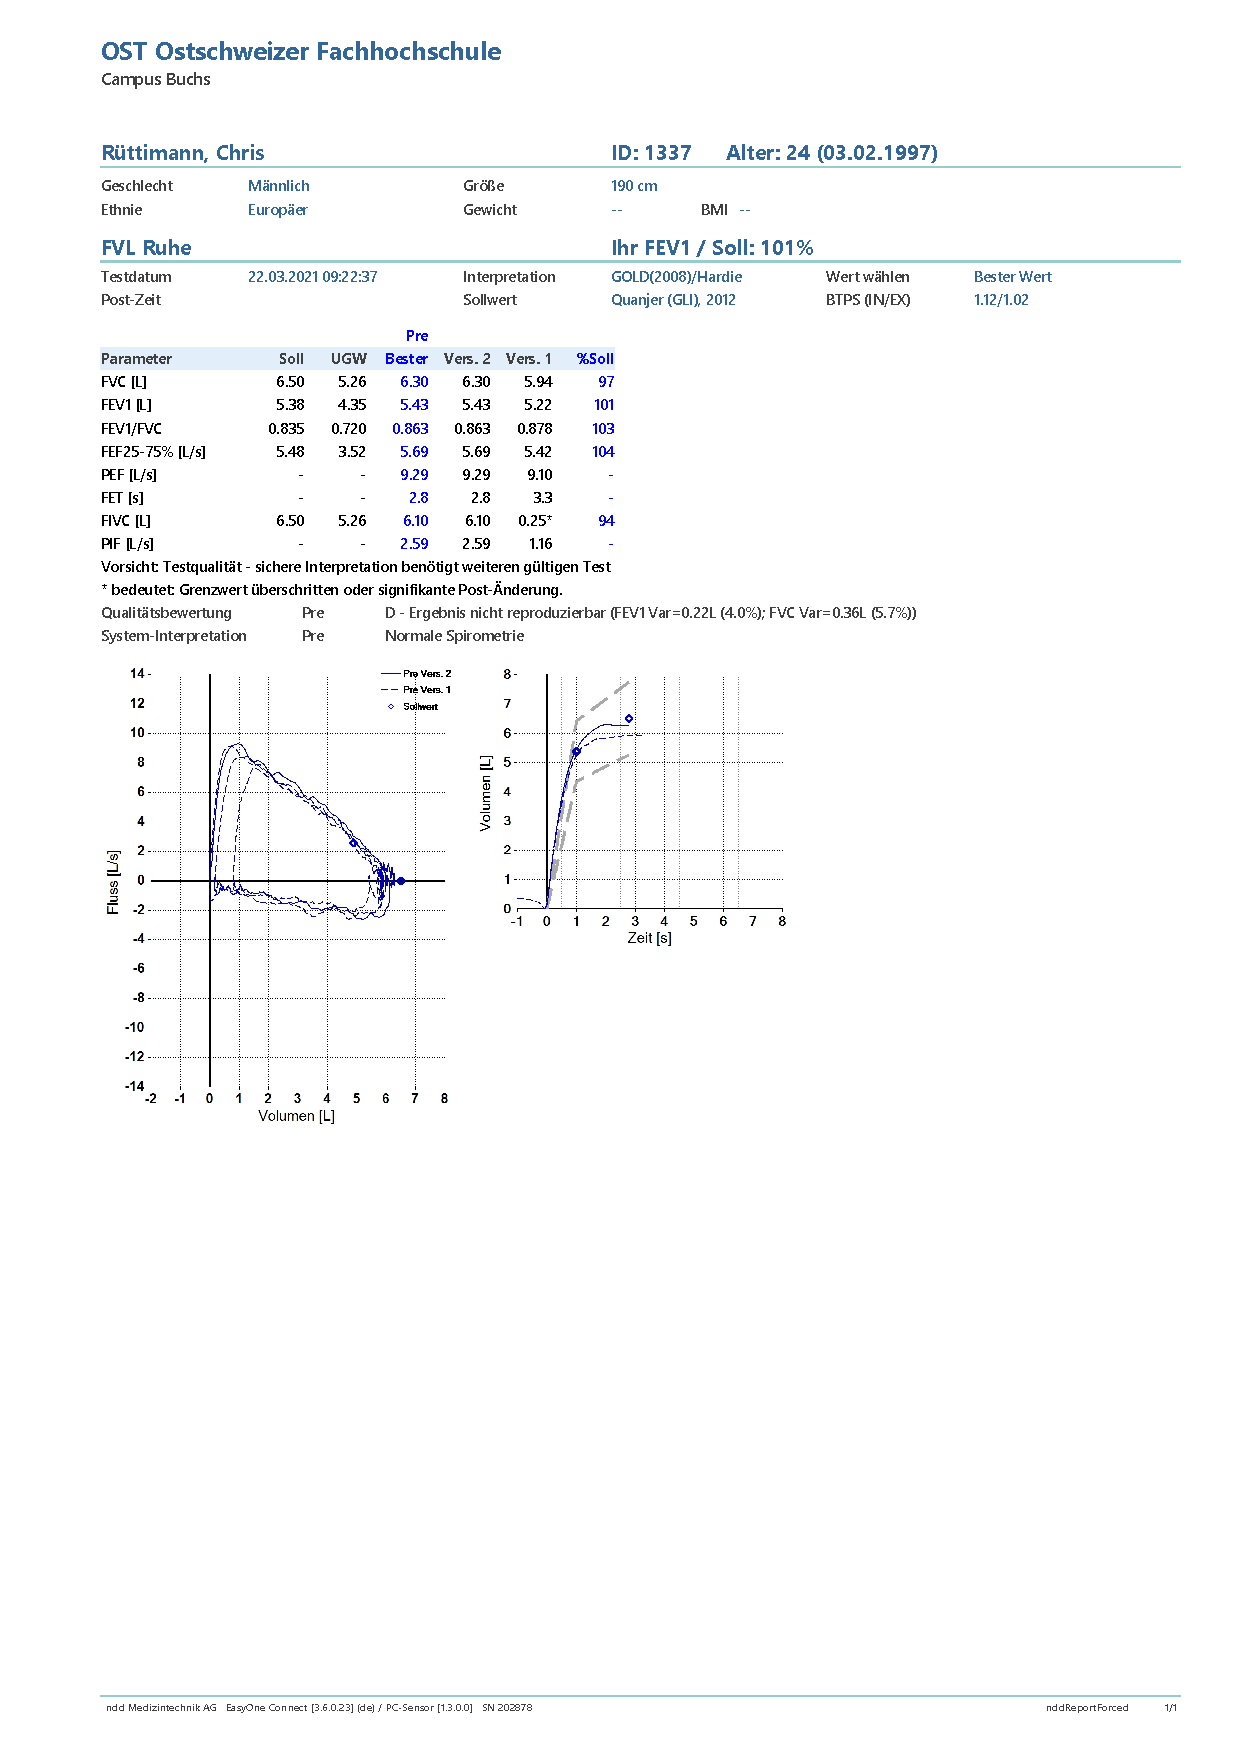
\includegraphics[clip, trim=1cm 10cm 0cm 11cm, width=15cm]{Dateien/Chris1.pdf}
        \caption{Chris, Messreihe 1}
    \end{figure}

    \begin{figure}[H]
        \centering
        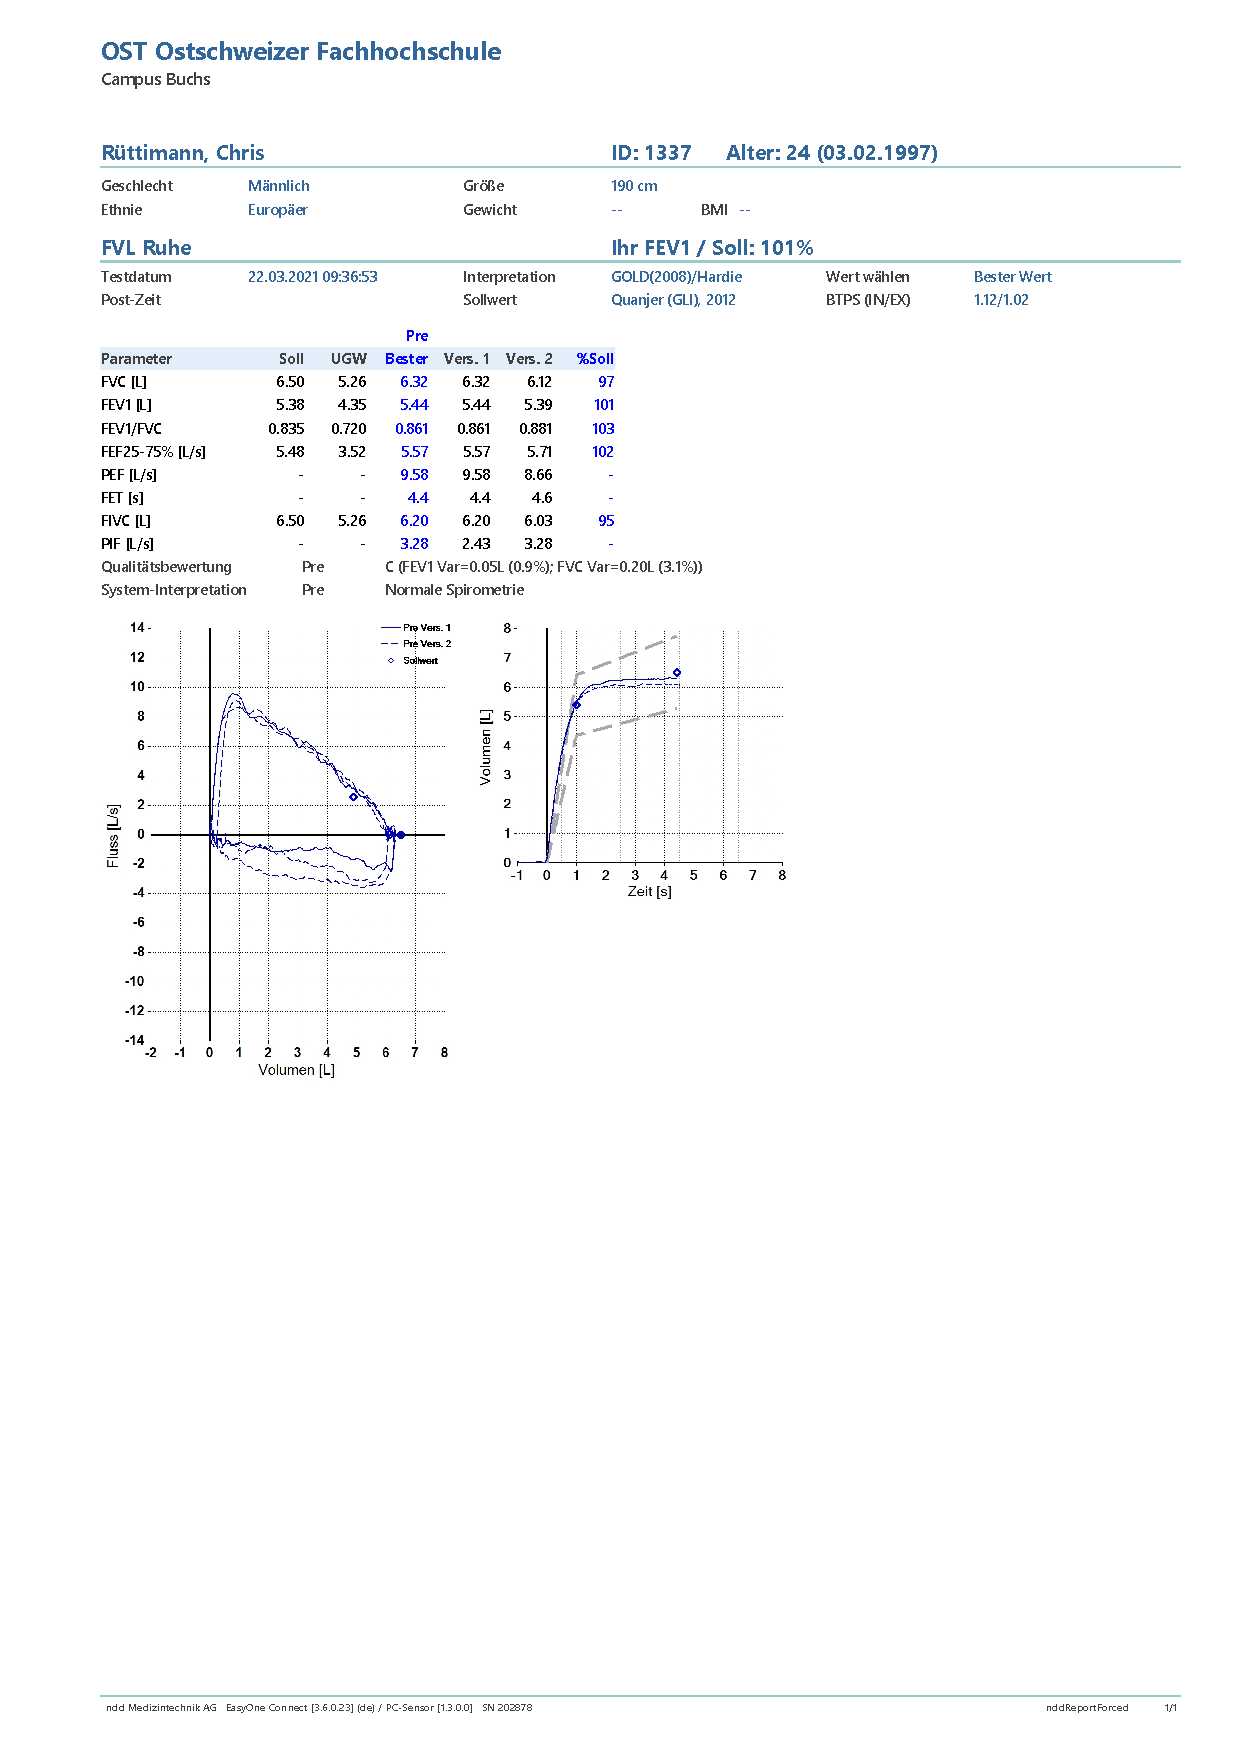
\includegraphics[clip, trim=1cm 10cm 0cm 11cm, width=15cm]{Dateien/Chris2.pdf}
        \caption{Chris, Messreihe 2}
    \end{figure}

    Aus den vollständigen Messergebnissen, siehe \autoref{sec:chris1} und \autoref{sec:chris2}, geht hervor, dass der
    Proband Rüttimann einen Tiffeneau-Index von 83\% bzw. 81\% erreicht hat.
    Diese beiden Werte weichen vom Sollwert, der 87\% beträgt, nur minimal ab.

    Die Flussvolumenkurve verläuft linear und ohne Knicke, das entspricht laut \autoref{Lungenkrankheiten} dem
    Normalbefund.
    %Die Messungen zeigen, dass bei Proband Chris die Lungenfunktion dem erwarteten Wert entsprechen.
    %Es können keine Abweichungen festgestellt werden, die auf eine Lungenkrankheit deuten.

    \pagebreak

    \subsection{Probandin Leona Köck}

    \begin{figure}[H]
        \centering
        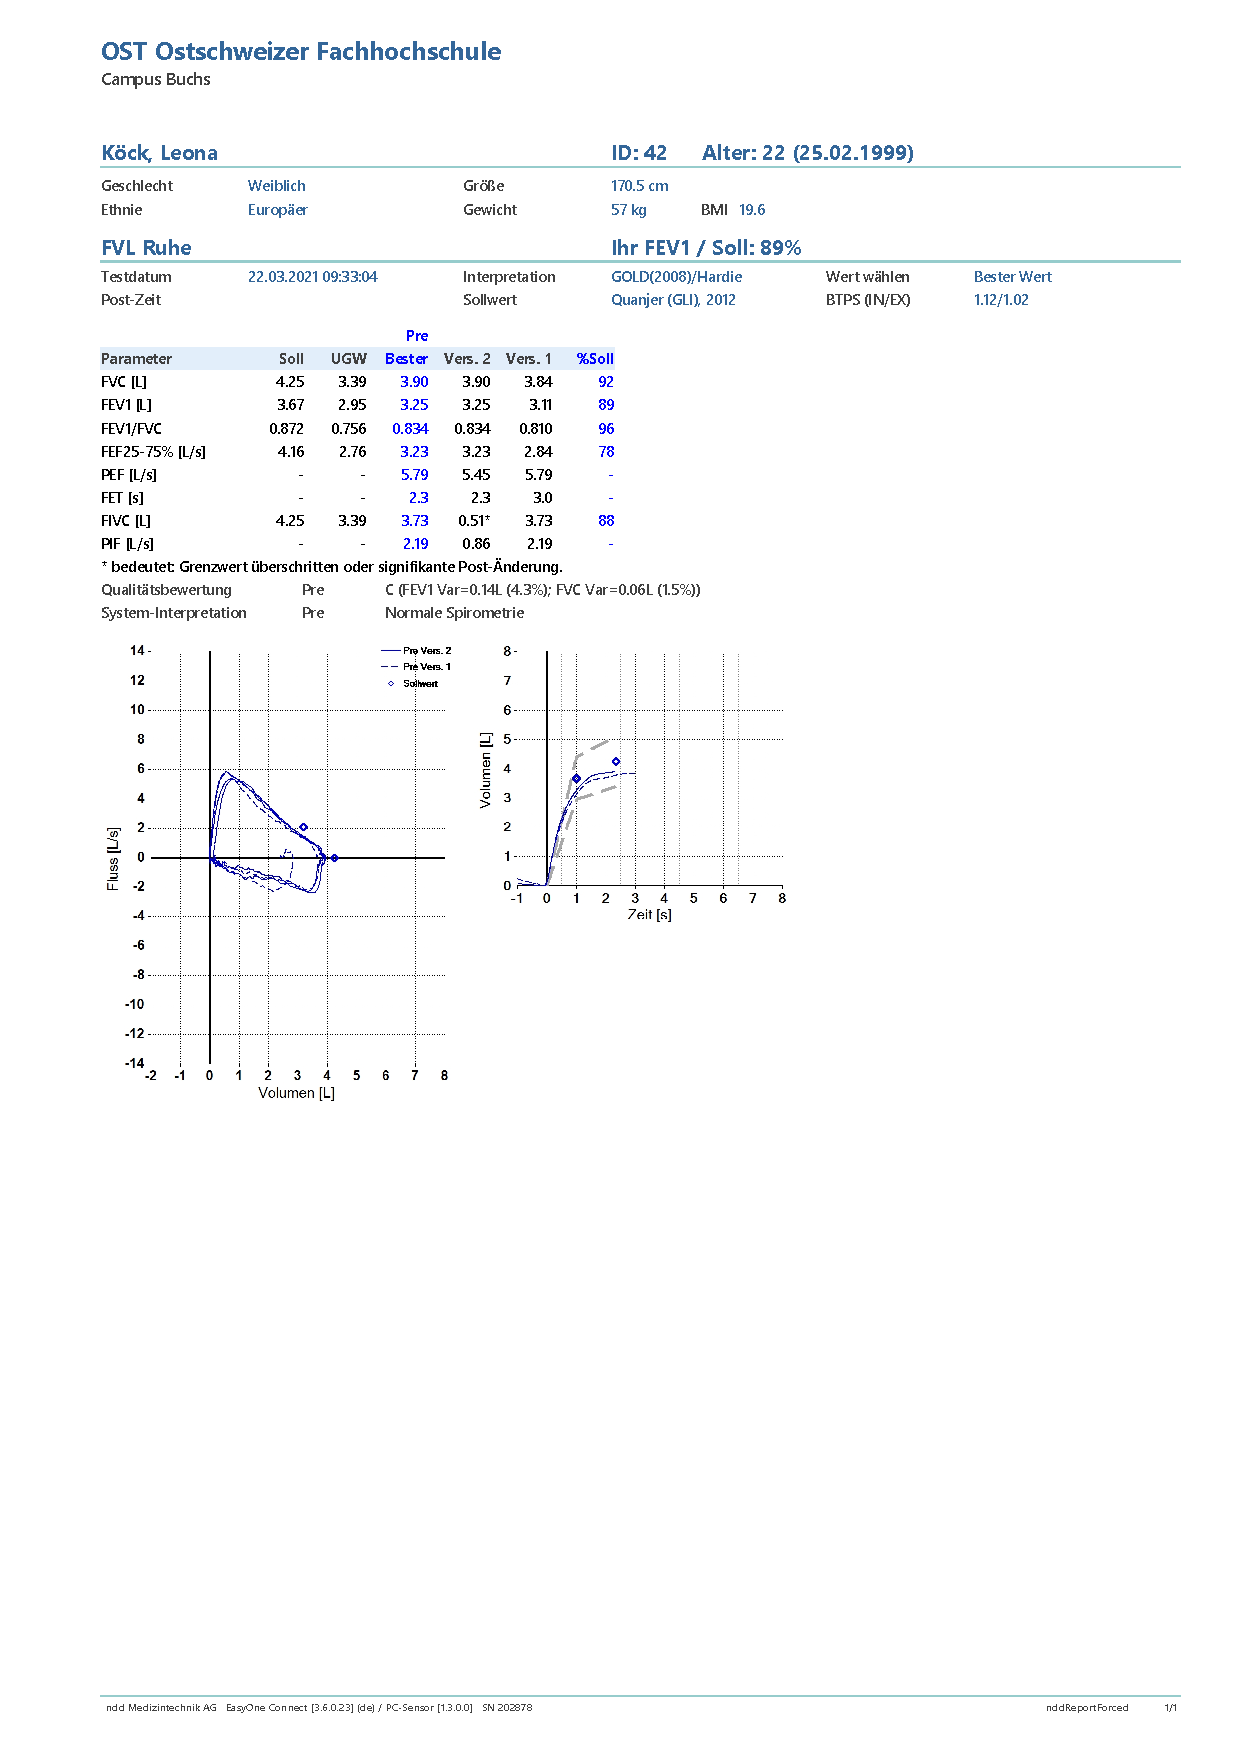
\includegraphics[clip, trim=1cm 10cm 0cm 10.6cm, width=15cm]{Dateien/Leona1.pdf}
        \caption{Leona, Messreihe 1}
    \end{figure}

        \begin{figure}[H]
        \centering
        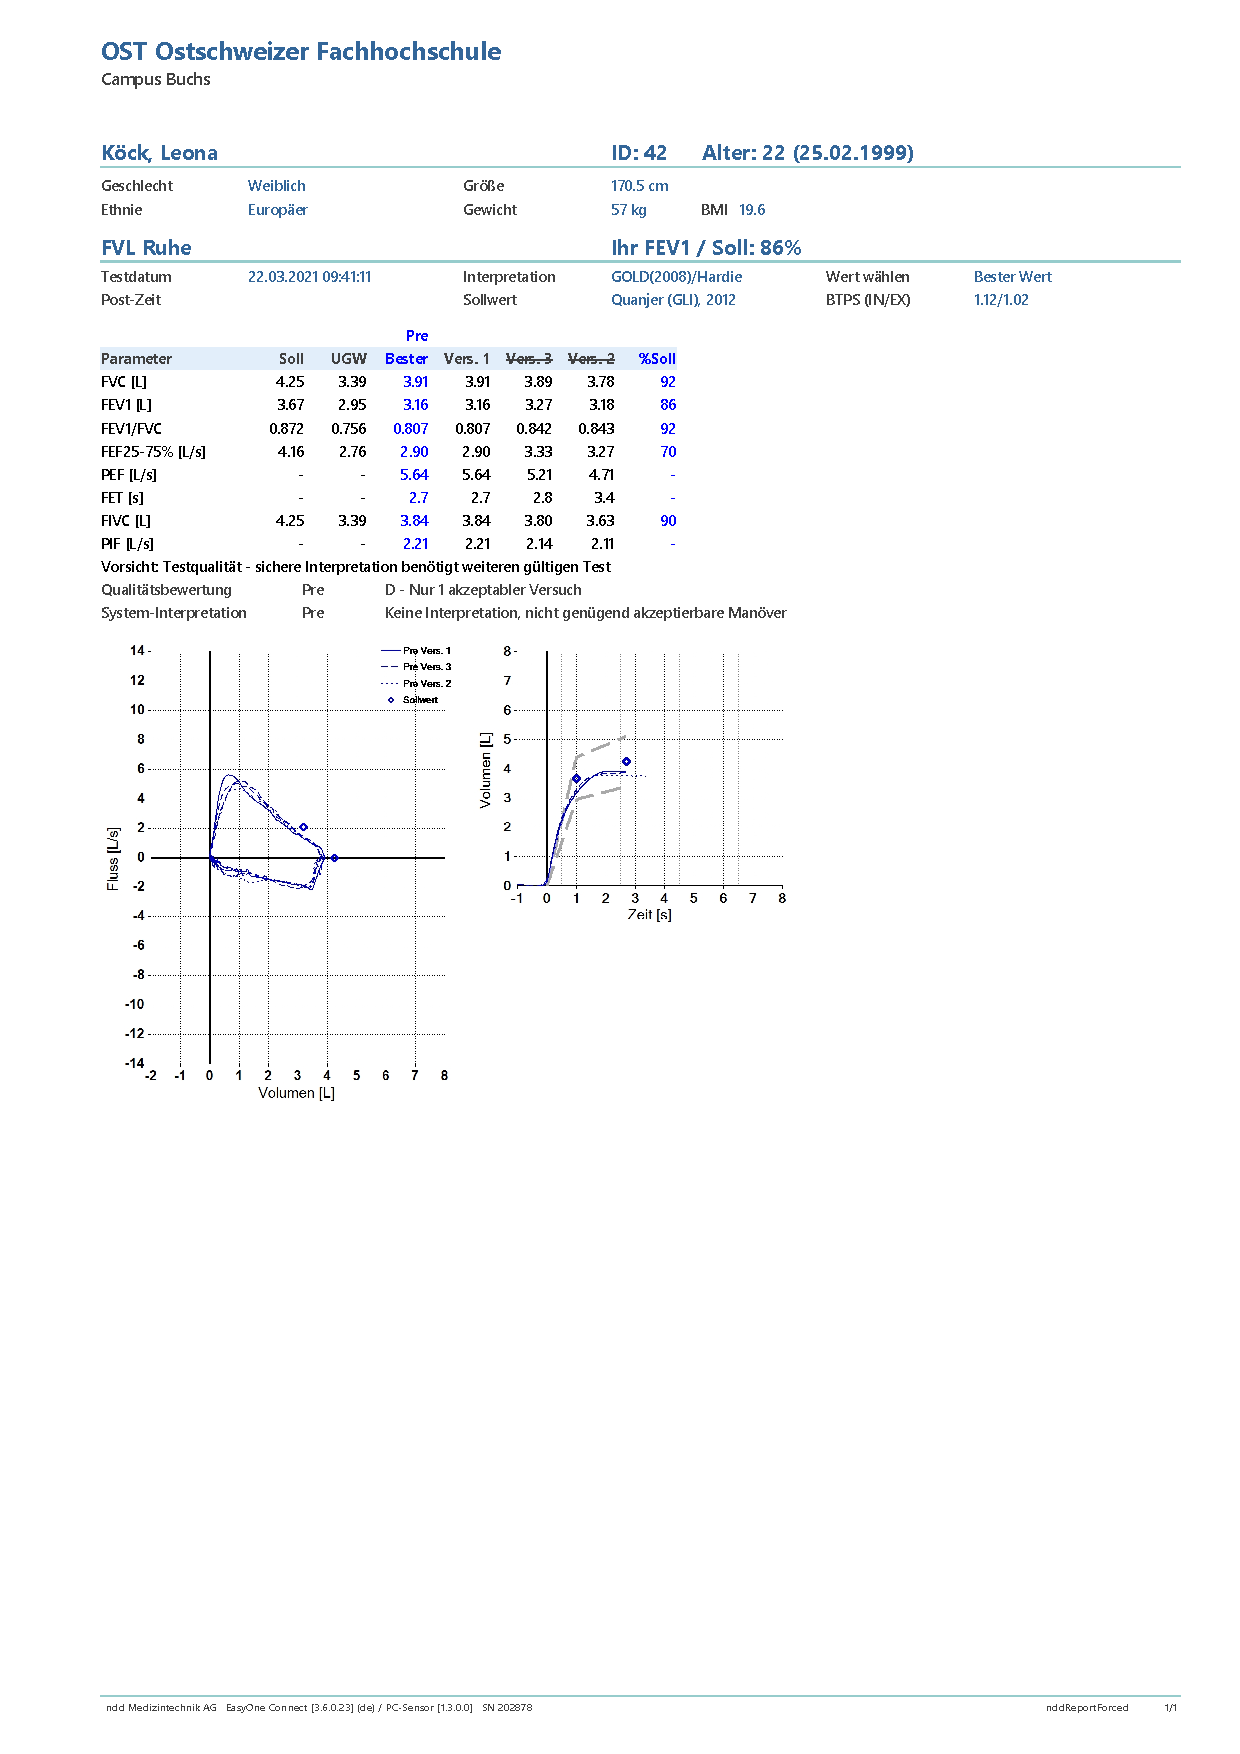
\includegraphics[clip, trim=1cm 10cm 0cm 10.6cm, width=15cm]{Dateien/Leona2.pdf}
        \caption{Leona, Messreihe 2}
        \end{figure}

    %Bei Probandin Leona ist eine sehr leichte Obstruktion erkennbar.
    %Es ist bekannt, dass ihr linker Lungenflügel etwas kleiner ist wie im Durchschnitt.
    % i han aber ka COPD :'(
    %todo leona1 wird nicht angezeigt

    Aus den vollständigen Messergebnissen, siehe \autoref{sec:leona1} und \autoref{sec:leona2}, geht hervor, dass die
    Probandin Köck einen Tiffeneau-Index von 80.7\% erreicht hat.
    Diese beiden Werte weichen vom Sollwert, der 87\% beträgt ein wenig ab.

    Vergleicht man die Messergebnisse von den zwei Probanden ist sehr auffällig, dass sich die absoluten Volumenwerte
    um ca. 2L unterscheiden.
    Das kommt daher, dass Frauen rund 25\,\% weniger Vitalkapazität haben als Männer.
    Zudem ist Herr Rüttimann mit einer Körpergrösse von 1.90\,m verhältnismässig gross, dementsprechend ist auch das
    Lungenvolumen grösser.

    %Die Flussvolumenkurve verläuft linear und ohne Knicke, das entspricht laut \autoref{lungenkrankheiten} dem
    %Normalbefund.

    \section{Lungenkrankheiten} \label{Lungenkrankheiten}

    \begin{figure}[H]
        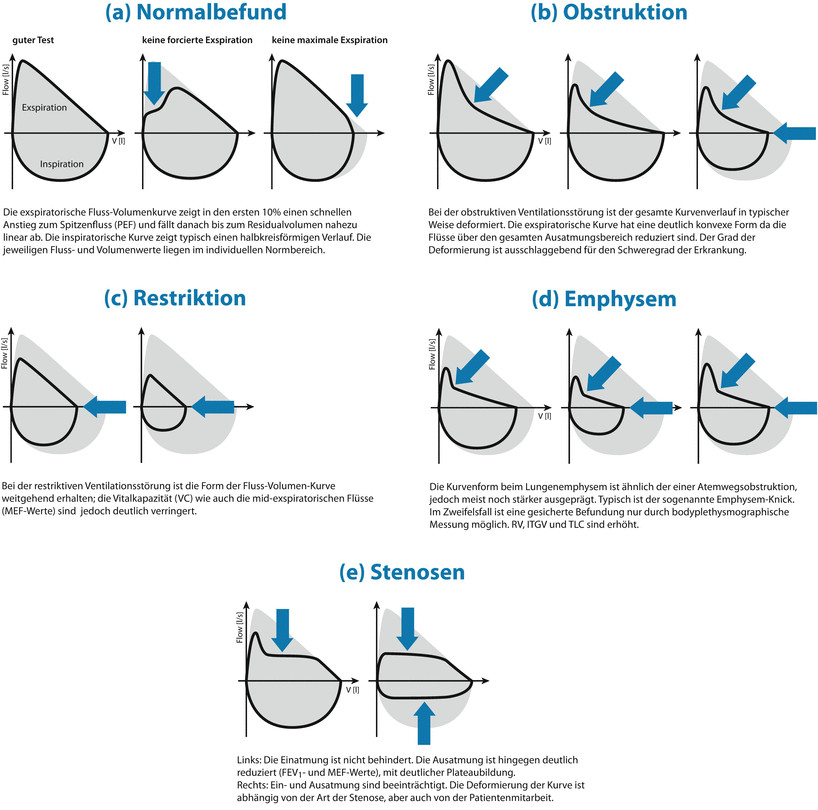
\includegraphics[width=15cm]{Dateien/Flusskurve.jpeg}
        \caption{Fluss-Volumenkurven, \cite{Flusskurven}}
        \label{fig:flusskurve}
    \end{figure}

    Abbildung \ref{fig:flusskurve} zeigt verschiedene Fluss-Volumenkurven und die dazugehörigen medizineschen Befunde.
    Bei einer Obstruktion ist die Kurve konvex deformiert, das kommt von einer dauerhaften Verengung der Atemwege die,
    wie man sieht, besonders die Ausatmung erschwert.
    Diese Krankheit ist auch bekannt unter COPD (\emph{Chronic Obstructive pulmonary disease}) oder zu deutsch
    \emph{Chronisch obstruktive Lungenerkrankung}.
    Bei einer Restriktiven Lungenkrankheit (Restriktion) ist die Entfaltung der Lunge behindert.
    Die Kurve hat dadurch dieselbe Form wie beim Normalbefund, ist aber kleiner.
    Eine weitere chronische Lungenkrankheit ist das Lungenemphysem, das mit Überblähung und Zerstörung der
    Lungenbläschen einhergeht.
    Dadurch wird die innere Fläche der Lunge kleiner und es kann, vor allem nach Belastung, nicht mehr ausreichend
    Sauerstoff aufgenommen oder abgegeben werden.
    Eine Stenose beschreibt die lokalisierte Verengung, die an verschiedenen Stellen wie der Trachea, der
    Bronchien oder in den Lungenarterien sein kann.
    Dafür gibt es mehrere unterschiedliche Auslöser, unter anderem an einem angeborenen Herzfehler oder durch
    künstliche Beatmung zustande kommen.
    %done: einzelne Sachen ein bisschen erklären (aka blabla)
    \pagebreak

    \section*{Eigenständigkeitserklärung}
    \addcontentsline{toc}{section}{Eigenständigkeitserklärung}

    Hiermit bestätigen wir, dass wir diesen Bericht selbstständig und ohne fremde Hilfe verfasst haben.
    Alle verwendeten Quellen wurden entsprechend dem APA-Standard gekennzeichnet.
    \\[3cm]


    \begin{figure}[H]
        
\includegraphics[width=4cm]{.././images/Unterschrift_Leona.png}
    \end{figure}
    \begin{tabular}{@{} l@{}}
        \hline \\
        \makebox[6cm]{Leona Köck}\\[2cm]
    \end{tabular}


    \begin{figure}[H]
        
\includegraphics[width=4cm]{.././images/Unterschrift_Chris.png}
    \end{figure}
    \begin{tabular}{@{} l@{}}
        \hline\\
        \makebox[6cm]{Chris Rüttimann}
    \end{tabular}

    \pagebreak
% ---------------------
% References
% ---------------------
    \printbibliography
    \addcontentsline{toc}{section}{Literaturverzeichnis}

% ---------------------
% List of figures
% ---------------------
%    \listoffigures
%    \addcontentsline{toc}{section}{Abbildungsverzeichnis}
%    \pagebreak

% ---------------------
% List of tables
% ---------------------
%\listoftables

% ---------------------
% Anhang
% ---------------------

\appendix

    \section{Messung 1 Chris}
    \label{sec:chris1}

    \begin{figure}[H]
        \hspace*{-3cm}
        \centering
        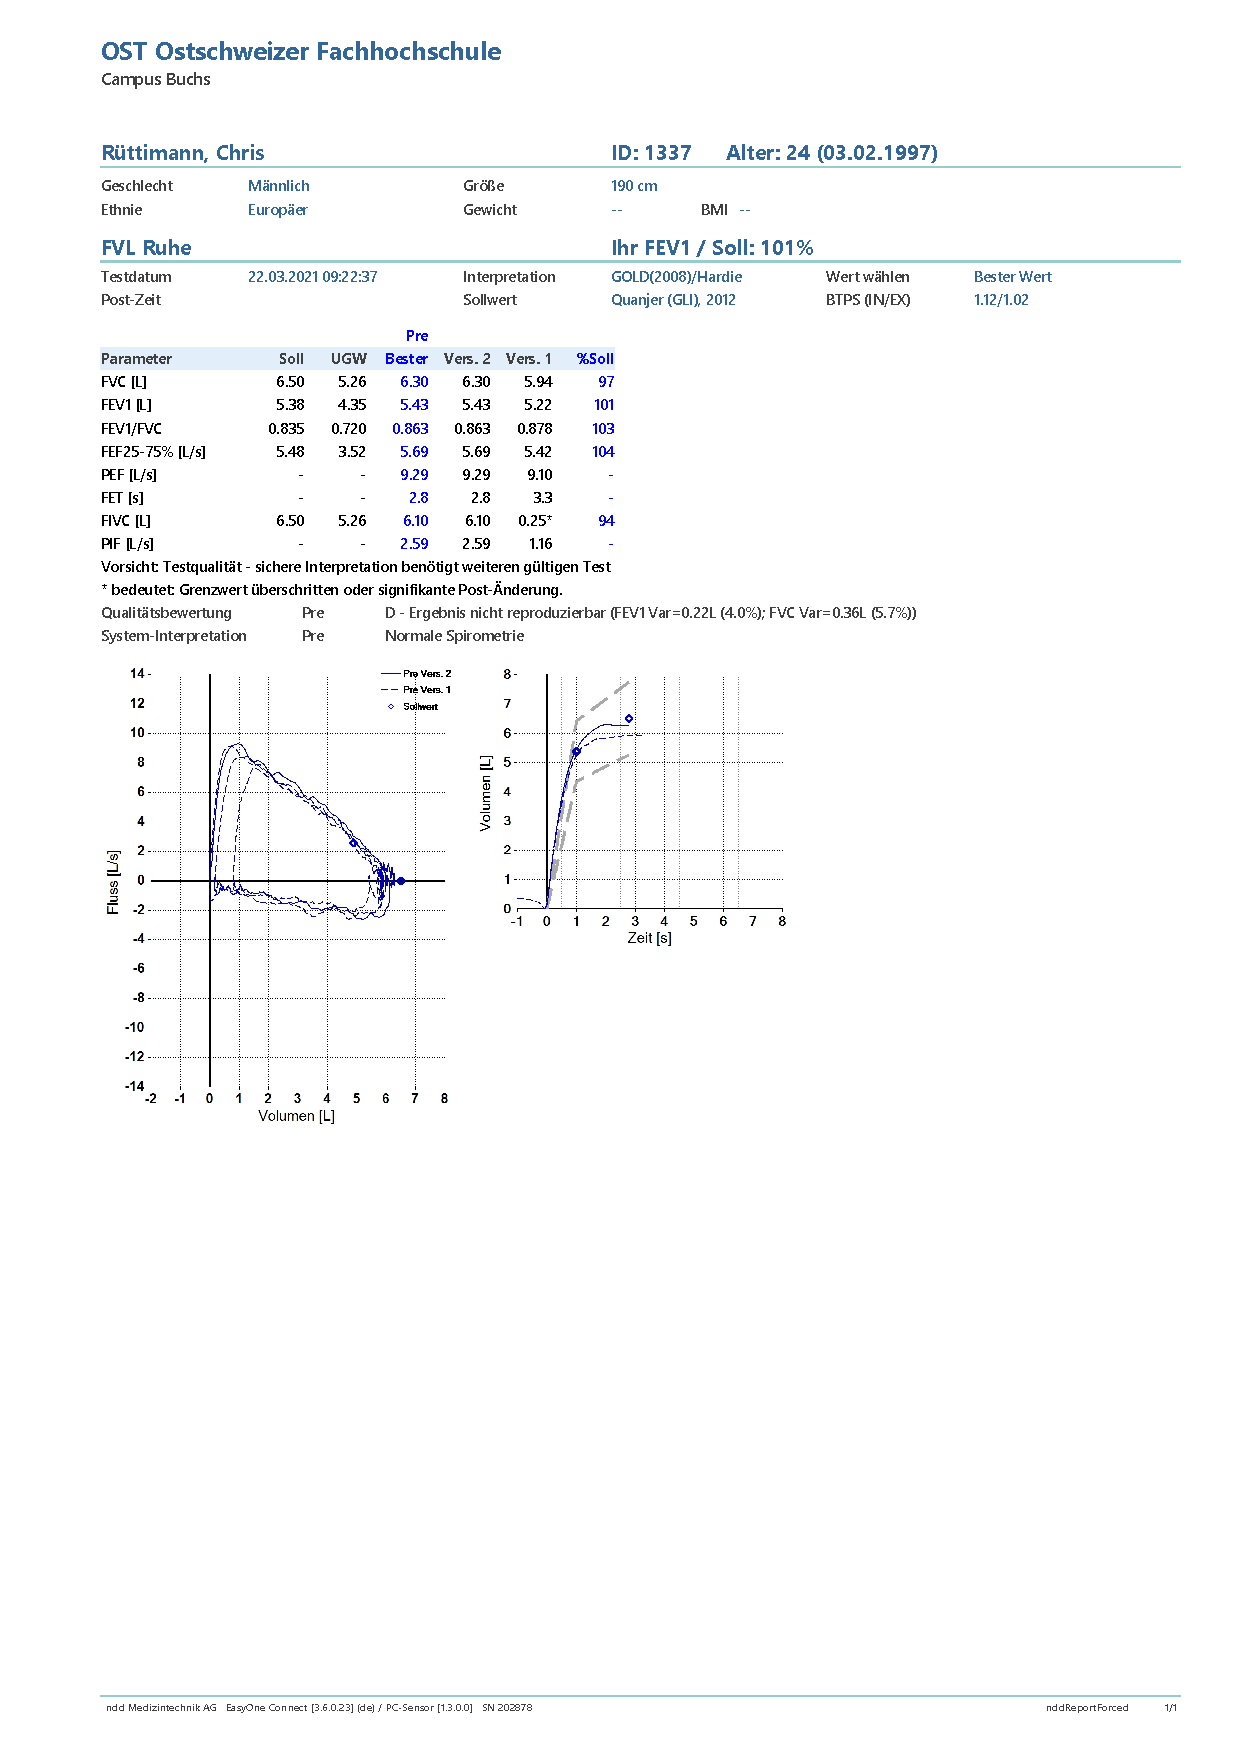
\includegraphics[clip, trim=0cm 10cm 0cm 0cm, width=1.4\textwidth]{Dateien/Chris1.pdf}
    \end{figure}

    \section{Messung 2 Chris}
    \label{sec:chris2}

    \begin{figure}[H]
        \hspace*{-3cm}
        \centering
        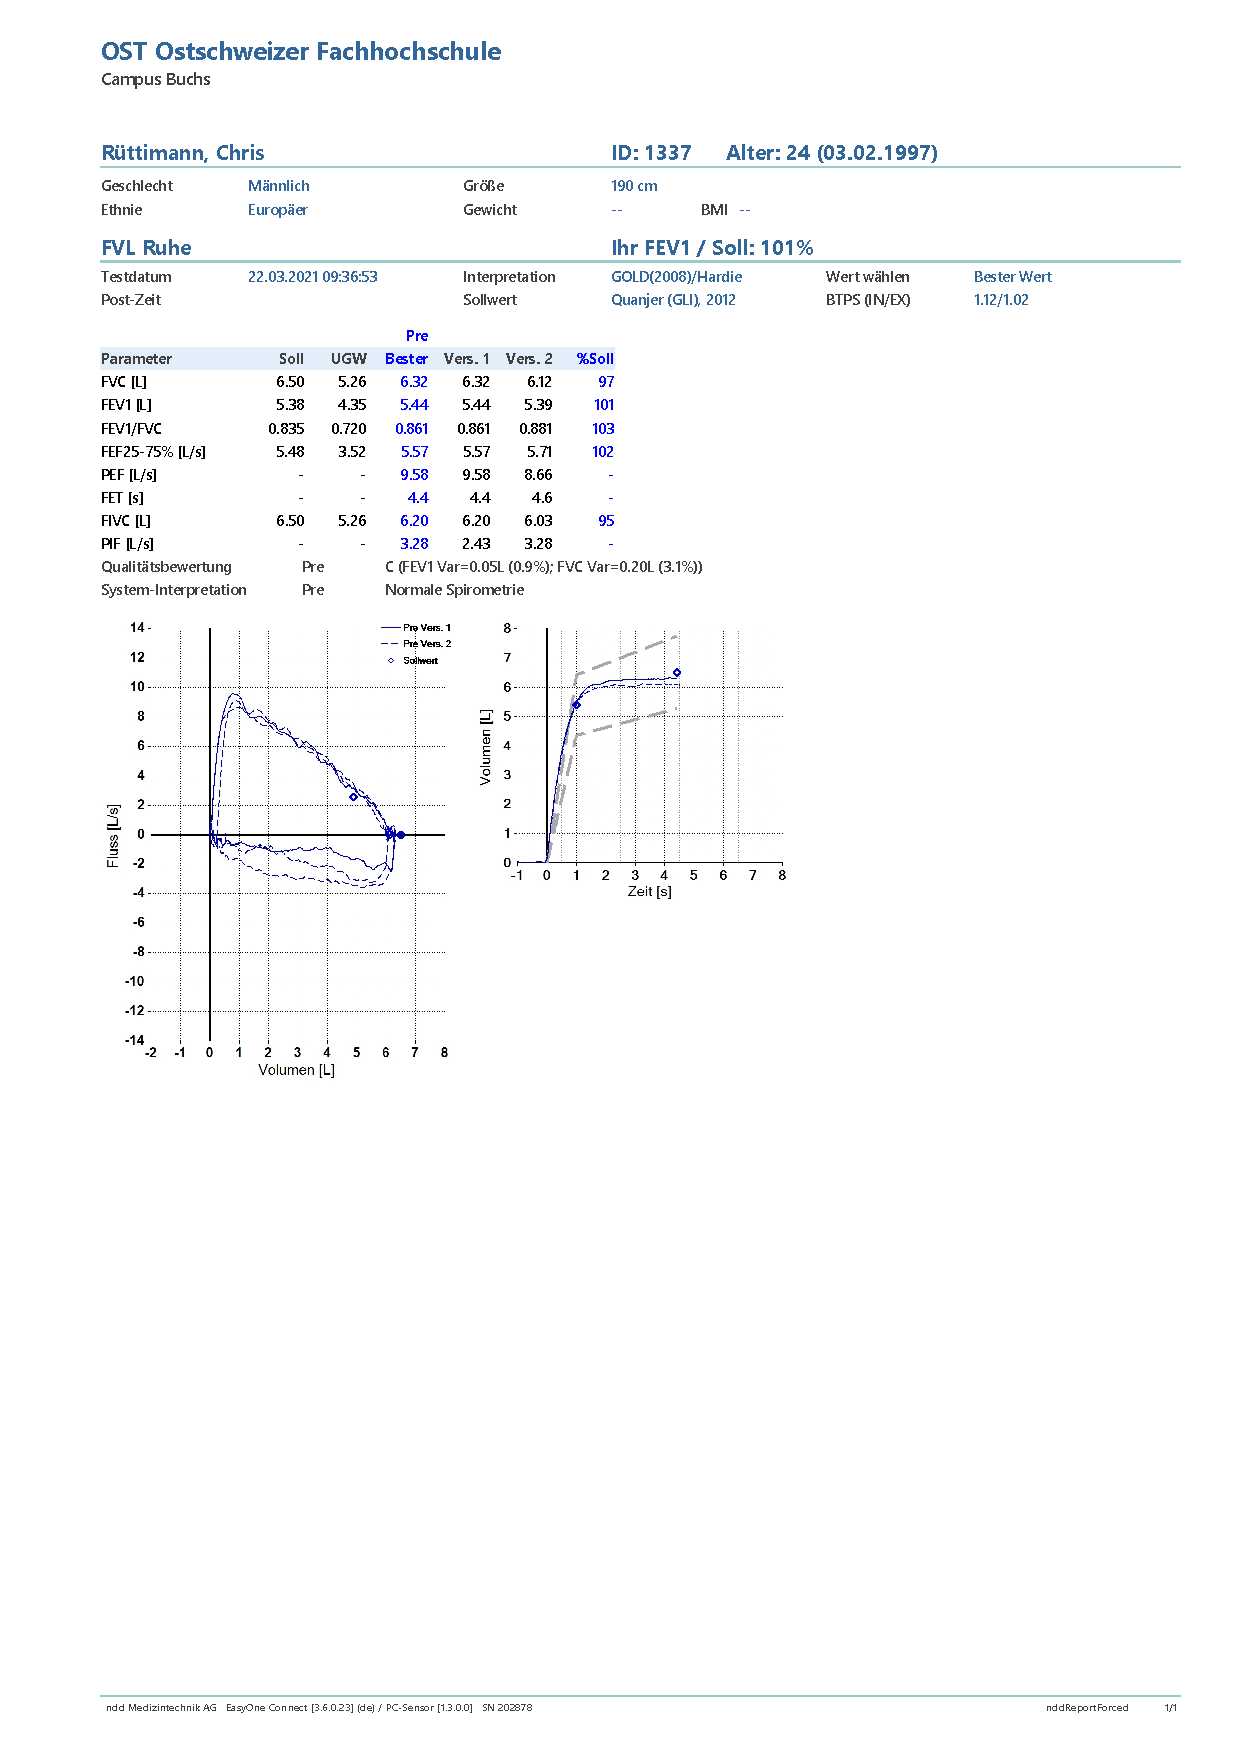
\includegraphics[clip, trim=0cm 10cm 0cm 0cm, width=1.4\textwidth]{Dateien/Chris2.pdf}
    \end{figure}

    \section{Messung 1 Leona}
    \label{sec:leona1}

    \begin{figure}[H]
        \hspace*{-3cm}
        \centering
        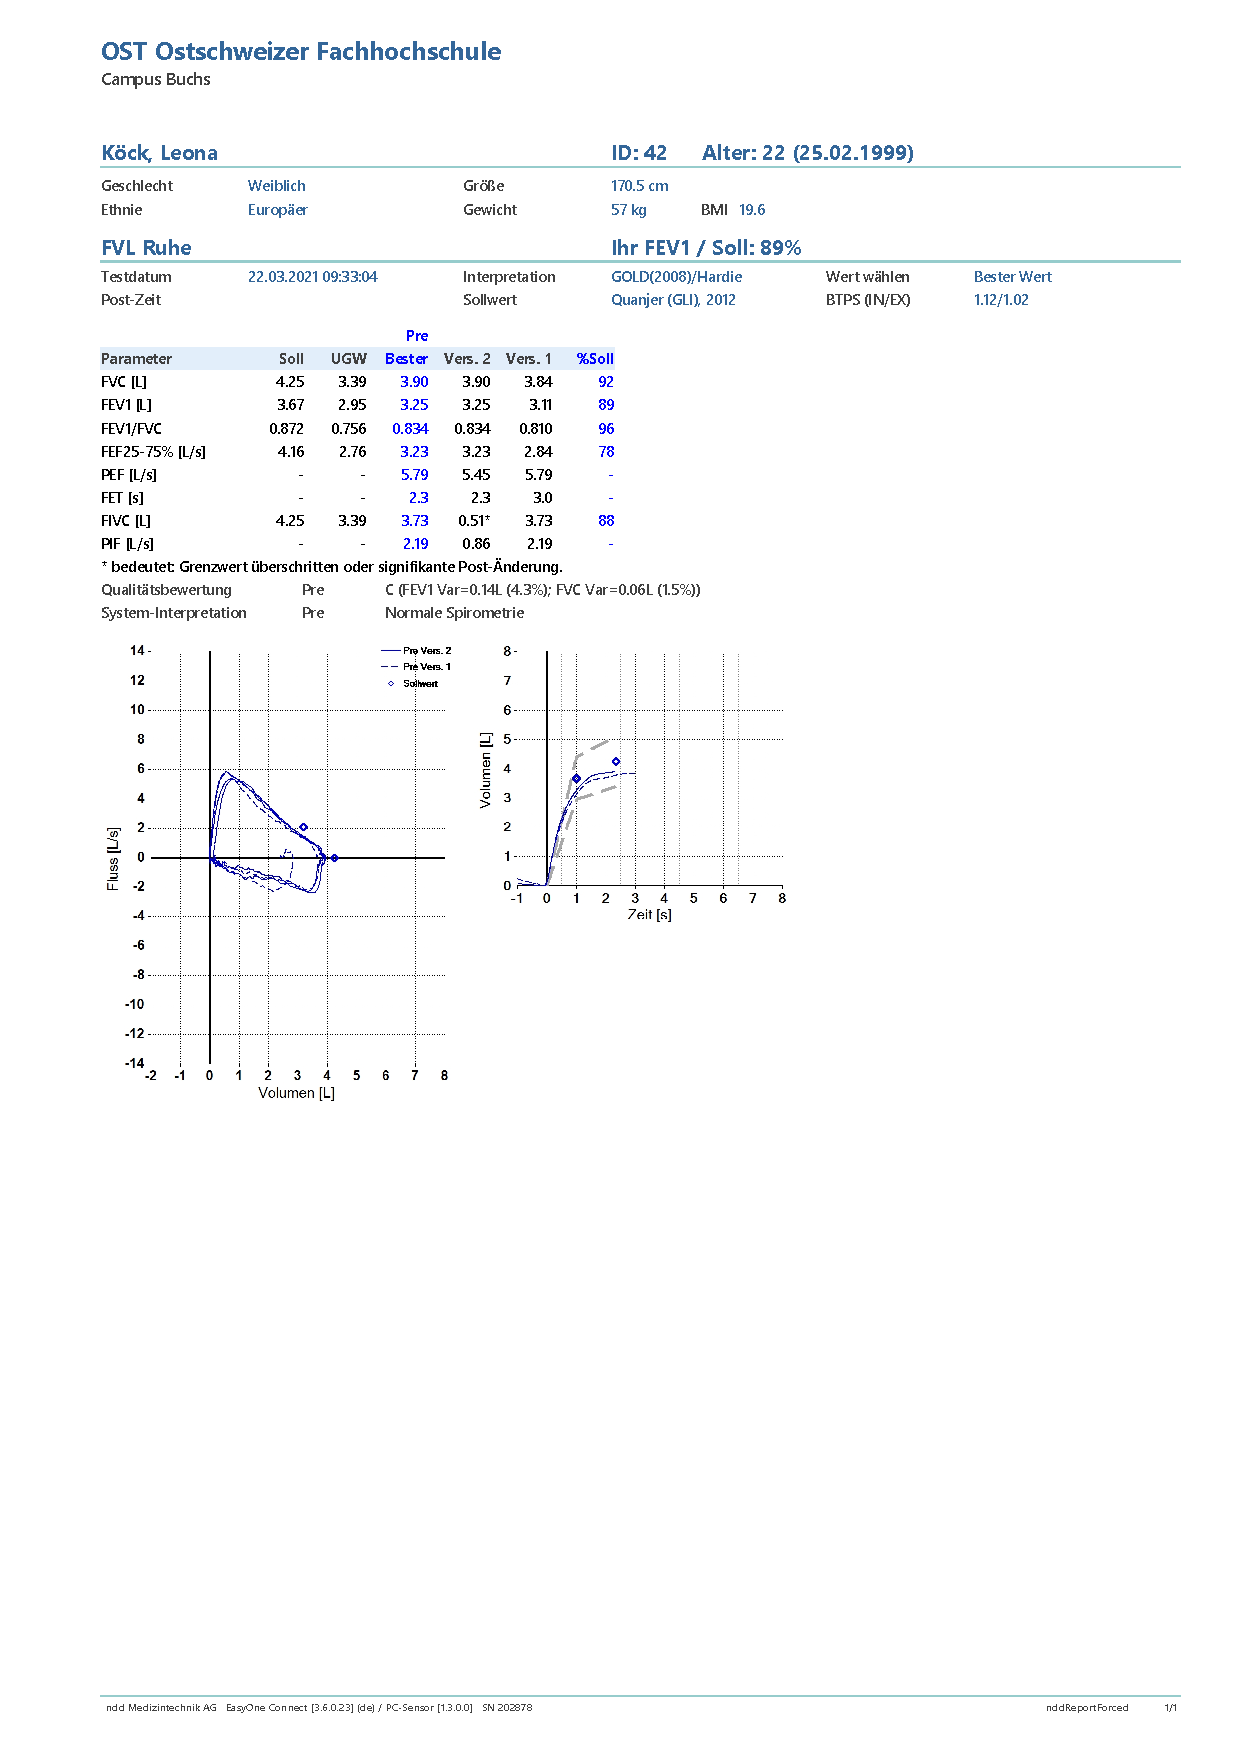
\includegraphics[clip, trim=0cm 10cm 0cm 0cm, width=1.4\textwidth]{Dateien/Leona1.pdf}
    \end{figure}

    \section{Messung 2 Leona}
    \label{sec:leona2}

    \begin{figure}[H]
        \hspace*{-3cm}
        \centering
        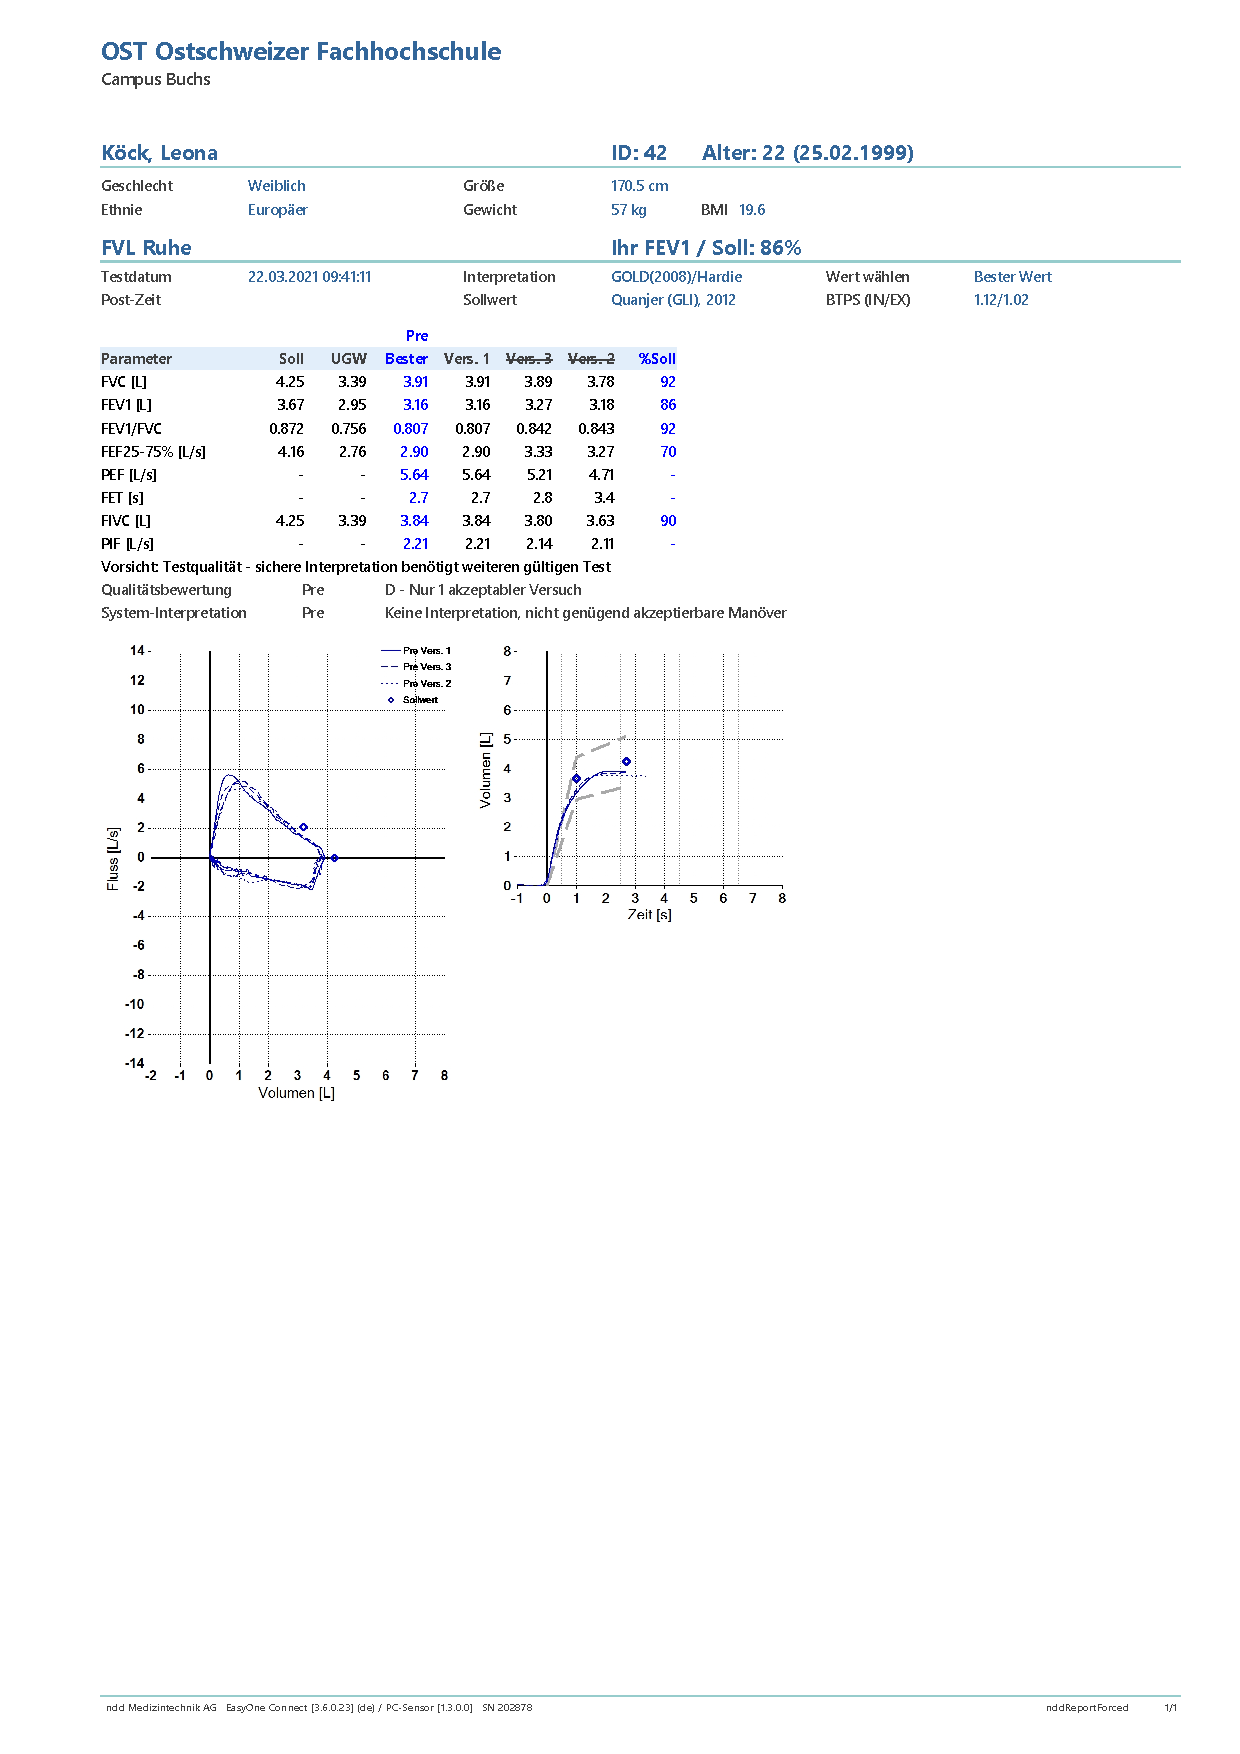
\includegraphics[clip, trim=0cm 10cm 0cm 0cm, width=1.4\textwidth]{Dateien/Leona2.pdf}
    \end{figure}

\end{document}